

\begin{figure}[t!]
\centering
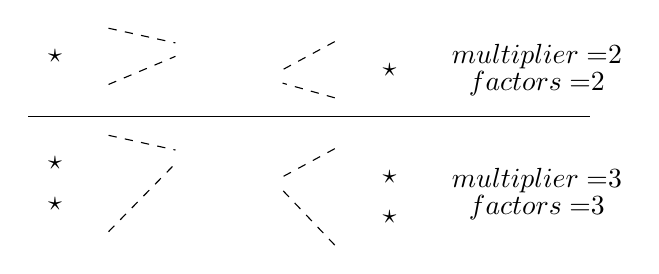
\begin{tikzpicture}[scale=0.17]

\pgfmathsetmacro{\height}{3}
\pgfmathsetmacro{\width}{8}
\pgfmathsetmacro{\leftOffset}{3}
\pgfmathsetmacro{\generalOffset}{0}

\volume{\generalOffset+ 10}{-2}{\generalOffset+10+\width}{2}

\Cvolume{\generalOffset+-\leftOffset}{2}{\generalOffset+-\leftOffset+\width}{3}{blue}
\Cvolume{\generalOffset+-\leftOffset}{-1}{\generalOffset+-\leftOffset+\width}{0}{blue}
\Cvolume{\generalOffset+10.05}{1.05}{\generalOffset+9.95+\width}{1.95}{blue}


\node[] at (\generalOffset+-\leftOffset+\width/2,1) {$\star$};

\draw [dashed] (\generalOffset+-\leftOffset+\width,3.1) -- (\generalOffset+10,2);
\draw [dashed] (\generalOffset+-\leftOffset+\width,-1.1) -- (\generalOffset+10,1);


\pgfmathsetmacro{\rightOffset}{4}

\Cvolume{\generalOffset+10+\width+\rightOffset}{1}{\generalOffset+10+2*\width+\rightOffset}{2}{black!30!green}
\Cvolume{\generalOffset+10+\width+\rightOffset}{-2}{\generalOffset+10+2*\width+\rightOffset}{-1}{black!30!green}
\Cvolume{\generalOffset+10.05}{-0.95}{\generalOffset+9.95+\width}{-0.05}{black!30!green}



\node[] at (\generalOffset+10+1.5*\width+\rightOffset,0) {$\star$};

\draw [dashed] (\generalOffset+10+\width + \rightOffset - 0.1,2.1) -- (\generalOffset+10+\width,0);
\draw [dashed] (\generalOffset+10+\width + \rightOffset - 0.1,-2.1) -- (\generalOffset+10+\width,-1);

\node[] at (37,+1) {$\text{multiplier=}2$};
\node[] at (37,-1) {$\text{factors=}2$};


\pgfmathsetmacro{\leftOffset}{3}
\pgfmathsetmacro{\generalOffset}{0}
\pgfmathsetmacro{\generalYOffset}{-8}

\volume{\generalOffset+ 10}{\generalYOffset+-2}{\generalOffset+10+\width}{\generalYOffset+2}

\Cvolume{\generalOffset+ 10-0.05}{\generalYOffset+1.05}{\generalOffset+9.95+\width}{\generalYOffset+2-0.05}{blue}
\Cvolume{\generalOffset+ 10}{\generalYOffset+-1+0.05}{\generalOffset+10+\width}{\generalYOffset-0.05}{black!30!green}


\Cvolume{\generalOffset+-\leftOffset}{\generalYOffset+2}{\generalOffset+-\leftOffset+\width}{\generalYOffset+3}{blue}
\Cvolume{\generalOffset+-\leftOffset}{\generalYOffset+-1}{\generalOffset+-\leftOffset+\width}{\generalYOffset+0}{blue}
\Cvolume{\generalOffset+-\leftOffset}{\generalYOffset+-4}{\generalOffset+-\leftOffset+\width}{\generalYOffset+-3}{blue}

\node[] at (\generalOffset+-\leftOffset+\width/2,\generalYOffset+1) {$\star$};
\node[] at (\generalOffset+-\leftOffset+\width/2,\generalYOffset+-2) {$\star$};


\draw [dashed] (\generalOffset+-\leftOffset+\width,\generalYOffset+3.1) -- (\generalOffset+10,\generalYOffset+2);
\draw [dashed] (\generalOffset+-\leftOffset+\width,\generalYOffset+-4.1) -- (\generalOffset+10,\generalYOffset+1);


\pgfmathsetmacro{\rightOffset}{4}

\Cvolume{\generalOffset+10+\width+\rightOffset}{\generalYOffset+1}{\generalOffset+10+2*\width+\rightOffset}{\generalYOffset+2}{black!30!green}
\Cvolume{\generalOffset+10+\width+\rightOffset}{\generalYOffset+-2}{\generalOffset+10+2*\width+\rightOffset}{\generalYOffset+-1}{black!30!green}
\Cvolume{\generalOffset+10+\width+\rightOffset}{\generalYOffset+-5}{\generalOffset+10+2*\width+\rightOffset}{\generalYOffset+-4}{black!30!green}

\node[] at (\generalOffset+10+1.5*\width+\rightOffset,\generalYOffset+0) {$\star$};
\node[] at (\generalOffset+10+1.5*\width+\rightOffset,\generalYOffset+-3) {$\star$};

\draw [dashed] (\generalOffset+10+\width + \rightOffset - 0.1,\generalYOffset+2.1) -- (\generalOffset+10+\width,\generalYOffset+0);
\draw [dashed] (\generalOffset+10+\width + \rightOffset - 0.1,\generalYOffset+-5.1) -- (\generalOffset+10+\width,\generalYOffset+-1);


\draw [] (\generalOffset-1,\generalYOffset+4.5) -- (\generalOffset+41,\generalYOffset+4.5);
\node[] at (\generalOffset+37,\generalYOffset-0.3) {$\text{multiplier=}3$};
\node[] at (\generalOffset+37,\generalYOffset-2.3) {$\text{factors=}3$};



\end{tikzpicture}
\vspace{-0.3cm}
    \caption{ Two LOST parametrizations of a conv1d layer with a single channel input making the layer weight a matrix of shape ({\rm n\_filters},{\rm filters\_length}). In {\bf both} cases, we use $K=R$ with value of $2$ as the {\bf top} and $3$ at the {\bf bottom} i.e. the resulting LOST layer has $2$ and $3$ times more parameters than the non over-parametrized counter-part. Note that padding is adjusted for the inter-filter convolutions to ensure that the final filter is of same length than the original layer. For multi-channel inputs, the same is applied to each of the ${\rm channels\_in}$ block of the conv1d layer weight.}
    \label{fig:codon1d}
\end{figure}
